
\section{Simulations}\label{sec-sim}


\subsection{\textcolor{red}{Small sample properties of the multiscale test}}\label{subsec-sim-multiscale}


In what follows, we investigate the performance of our multiscale test and compare it to the dependent SiZer methods from \cite{Rondonotti2004}, \cite{Rondonotti2007} and \cite{ParkHannigKang2009}. We consider the following versions of our multiscale test and SiZer:
\begin{itemize}[leftmargin=1.25cm]

\item[$\mathcal{T}_{\text{MS}}$:] our multiscale test with the statistic $\widehat{\Psi}_T = \max_{h \in H_T} \{ \widehat{\Psi}_T(h) - \lambda(h) \}$, where $\widehat{\Psi}_T(h) = \max_{u \in U_T} |\widehat{\psi}_T(u,h) / \widehat{\sigma}|$. Here and in what follows, we write $\mathcal{G}_T = U_T \times H_T$, where $U_T$ is the set of locations and $H_T$ the set of bandwidths.  

\item[$\mathcal{T}_{\text{UC}}$:] the uncorrected version of our multiscale test with the test statistic $\widehat{\Psi}_{T,\text{uncorrected}} = \max_{h \in H_T} \widehat{\Psi}_T(h)$, which was already introduced in \eqref{multiscale-stat-uncorrected}. The uncorrected test is carried out in exactly the same way as $\mathcal{T}_{\text{MS}}$. The only difference is that the correction terms $\lambda(h)$ are removed. 

\item[$\mathcal{T}_{\text{RW}}$:] a row-wise (or scale-wise) version of our multiscale test as briefly mentioned in Section \ref{subsec-method-comparison}. This version carries out a test scale-wise, that is, separately for each scale $h \in H_T$ based on the statistic $\widehat{\Psi}_T(h)$. Note: (i) For each $h \in H_T$, the test based on $\widehat{\Psi}_T(h)$ can be performed in the same way as the multiscale test $\mathcal{T}_{\text{MS}}$, since it is a degenerate version of the latter with the set of scales $H_T$ replaced by the singleton $\{h\}$. (ii) It does not matter whether we correct the statistic $\widehat{\Psi}_T(h)$ by subtracting $\lambda(h)$ or not, since $\lambda(h)$ acts as a fixed constant when only one bandwidth $h$ is taken into account. 

\item[$\mathcal{T}_{\text{SiZer}}$:] the row-wise version of dependent SiZer as developed in \cite{Rondonotti2004}, \cite{Rondonotti2007} and \cite{ParkHannigKang2009}. We do not consider a global version of dependent SiZer since such a version was not introduced in the aforementioned papers. 

\end{itemize}


The simulation setup is as follows: We generate data from the model $Y_{t,T} = m(t/T) + \varepsilon_t$ for different trends $m$, error processes $\{\varepsilon_t\}$ and sample sizes $T$. The error terms are supposed to have the AR($1$) structure $\varepsilon_t = a_1 \varepsilon_{t-1} + \eta_t$, where $a_1 \in \{-0.9,-0.5,-0.25, \linebreak 0.25,0.5,0.9\}$, $\eta_t$ are i.i.d.\ standard normal and the AR order $p^*=1$ is treated as known. To simulate data under the null, we let $m$ be a constant function. In particular, we set $m = 0$ without loss of generality. To generate data under the alternative, we consider different non-constant trend functions which are specified below. For each model specification, we simulate $S=1000$ data samples and carry out the tests $\mathcal{T}_{\text{MS}}$, $\mathcal{T}_{\text{UC}}$, $\mathcal{T}_{\text{RW}}$ and $\mathcal{T}_{\text{SiZer}}$ for each simulated sample. 


To implement our multiscale test $\mathcal{T}_{\text{MS}}$, we choose $K$ to be an Epanechnikov kernel and set $\mathcal{G}_T = U_T \times H_T$, where 
\begin{align*}
U_T & = \big\{ u \in [0,1]: u = \textstyle{\frac{5t}{T}} \text{ for some } t \in \naturals \big\} \\
H_T & = \big\{ h \in \big[ \textstyle{\frac{\log T}{T}}, \textstyle{\frac{1}{4}} \big]:  h = \textstyle{\frac{5\ell}{T}} \text{ for some } t \in \naturals \big\}. 
\end{align*}
We thus take into account all locations $u$ on an equidistant grid $U_T$ with step length $5/T$ and all bandwidths $h=5/T, 10/T, 15/T,\ldots$ with $\log T /T \le h \le 1/4$. Note that the lower bound $\log T / T$ is motivated by \ref{C-h} which requires that $\log T /T \ll h$ for all scales $h \in H_T$ (given that all moments of $\varepsilon_t$ exist). As a robustness check, we have re-run the simulations for a number of other grids. As the results are very similar, we do however not report them here. 
To estimate the long-run error variance $\sigma^2$, we apply the procedure from Section \ref{sec-error-var} with $\overline{r}=10$ and the following choices of $q$: For $a_1 \in \{-0.5,-0.25,0.25,0.5\}$, we set $q = 25$. As already discussed in Section \ref{sec-error-var}, this should be an appropriate choice for AR(1) errors that are not too strongly correlated, in particular, for $a_1 \in \{-0.5,-0.25,0.25,0.5\}$. When the errors are very strongly correlated, larger values of $q$ are required to produce precise estimates of $\sigma^2$. In the case of AR($1$) errors with $a_1 \in \{-0.9,0.9\}$, we thus set $q = 50$. The dependence of our long-run variance estimator on the tuning parameters $q$ and $\overline{r}$ is explored more systematically in Section \ref{subsec-sim-lrv}. 
To compute the critical values of the multiscale test $\mathcal{T}_{\text{MS}}$, we simulate $5000$ values of the statistic $\Phi_T$ defined in Section \ref{subsec-method-test} and compute their empirical $(1-\alpha)$ quantile $q_T(\alpha)$. The uncorrected and row-wise versions $\mathcal{T}_{\text{UC}}$ and $\mathcal{T}_{\text{RW}}$ of our multiscale test are implemented analogously. The SiZer test is implemented as described in \cite{ParkHannigKang2009}. The details are summarized in Section S.3 of the Supplementary Material. 


\subsubsection{Size simulations}\label{subsec-sim-multiscale-size} 


The first part of our simulation study investigates the size properties of the four tests $\mathcal{T}_{\text{MS}}$, $\mathcal{T}_{\text{UC}}$, $\mathcal{T}_{\text{RW}}$ and $\mathcal{T}_{\text{SiZer}}$ under the null that the trend $m$ is constant. To start with, we focus on the multiscale test $\mathcal{T}_{\text{MS}}$. Table \ref{tab:sim:size:MS1} reports the actual size of $\mathcal{T}_{\text{MS}}$ for the AR parameters $a_1 \in \{-0.5,-0.25,0.25,0.5\}$, which is computed as the number of simulations in which $\mathcal{T}_{\text{MS}}$ rejects the null divided by the total number of simulations. As can be seen, the actual size of the multiscale test $\mathcal{T}_{\text{MS}}$ is fairly close to the nominal target $\alpha$ for all the considered AR parameters and sample sizes. Hence, the test has approximately the correct size.


\begin{table}[t!]
\footnotesize{
\caption{Size of $\mathcal{T}_{\text{MS}}$ for the AR parameters $a_1 \in \{-0.5,-0.25,0.25,0.5\}$.}\label{tab:sim:size:MS1}
\newcolumntype{C}[1]{>{\hsize=#1\hsize\centering\arraybackslash}X}
\newcolumntype{Z}{>{\centering\arraybackslash}X}
\begin{tabularx}{\textwidth}{l Z@{\hskip 6pt}Z@{\hskip 6pt}Z Z@{\hskip 6pt}Z@{\hskip 6pt}Z Z@{\hskip 6pt}Z@{\hskip 6pt}Z Z@{\hskip 6pt}Z@{\hskip 6pt}Z} 
\toprule
 & \multicolumn{3}{c}{$a_1 = -0.5$} & \multicolumn{3}{c}{$a_1 = -0.25$} & \multicolumn{3}{c}{$a_1 = 0.25$} & \multicolumn{3}{c}{$a_1 = 0.5$} \\
\cmidrule[0.4pt]{2-4} \cmidrule[0.4pt]{5-7} \cmidrule[0.4pt]{8-10} \cmidrule[0.4pt]{11-13} 
 & \multicolumn{3}{c}{nominal size $\alpha$} &\multicolumn{3}{c}{nominal size $\alpha$} & \multicolumn{3}{c}{nominal size $\alpha$} & \multicolumn{3}{c}{nominal size $\alpha$} \\
 & 0.01 & 0.05 & 0.1  &  0.01 & 0.05 & 0.1  &  0.01 & 0.05 & 0.1  &  0.01 & 0.05 & 0.1 \\
\cmidrule[0.4pt]{1-13}
$T=250$  &  0.013 & 0.044 & 0.088  & 0.010 & 0.047 & 0.090  & 0.012 & 0.046 & 0.087  & 0.010 & 0.044 & 0.077 \\ 
$T=500$  &  0.010 & 0.045 & 0.087  & 0.008 & 0.040 & 0.087  & 0.007 & 0.047 & 0.094  & 0.007 & 0.051 & 0.110 \\ 
$T=1000$ &  0.009 & 0.049 & 0.108  & 0.010 & 0.047 & 0.106  & 0.009 & 0.052 & 0.100  & 0.010 & 0.055 & 0.093 \\ 
\bottomrule
\end{tabularx}}
\end{table}


\begin{table}[t!]
\centering
\footnotesize{
\caption{Size of $\mathcal{T}_{\text{MS}}$ for the AR parameters $a_1 \in \{-0.9,0.9\}$.}\label{tab:sim:size:MS2}
\newcolumntype{C}[1]{>{\hsize=#1\hsize\centering\arraybackslash}X}
\newcolumntype{Z}{>{\centering\arraybackslash}X}
\begin{tabularx}{\textwidth}{l@{\hskip20pt} Z@{\hskip 6pt}Z@{\hskip 6pt}Z@{\hskip 6pt}Z@{\hskip 6pt}Z@{\hskip 20pt}Z@{\hskip 6pt}Z@{\hskip 6pt}Z@{\hskip 6pt}Z@{\hskip 6pt}Z}
\toprule
 & \multicolumn{5}{c}{$a_1 = -0.9$} & \multicolumn{5}{c}{$a_1 = 0.9$} \\
\cmidrule[0.4pt]{2-11}   
 & \multicolumn{5}{c}{sample size $T$} & \multicolumn{5}{c}{sample size $T$} \\
 & 250 & 500 & 1000 & 2000 & 3000  &  250 & 500 & 1000 & 2000 & 3000 \\
\cmidrule[0.4pt]{1-11}
$\alpha=0.01$ &  0.041 & 0.016 & 0.018 & 0.014 & 0.014  & 0.001 & 0.016 & 0.018 & 0.016 & 0.015 \\ 
$\alpha=0.05$ &  0.109 & 0.086 & 0.063 & 0.057 & 0.062  & 0.017 & 0.057 & 0.054 & 0.056 & 0.058 \\ 
$\alpha=0.1$  &  0.171 & 0.153 & 0.130 & 0.110 & 0.114  & 0.034 & 0.094 & 0.096 & 0.099 & 0.107 \\ 
\bottomrule
\end{tabularx}}
\end{table}


In Table \ref{tab:sim:size:MS1}, we have explored the size of $\mathcal{T}_{\text{MS}}$ when the error terms are moderately autocorrelated. The case of strongly autocorrelated errors is investigated in Table \ref{tab:sim:size:MS2}, where we consider AR($1$) errors with $a_1 \in \{-0.9,0.9\}$. We first discuss the results for the negative AR parameter $a_1=-0.9$. As can be seen, the size numbers are substantially upward biased for small sample sizes, in particular, for $T=250$ and $T=500$. As the sample size increases, this upward bias diminishes and the size numbers stabilize around their target $\alpha$. In particular, for $T \ge 1000$, the size numbers give a decent approximation to $\alpha$. An analogous picture arises for the positive AR parameter $a_1=0.9$. However, the size numbers are downward rather than upward biased for small sample sizes $T$ and the size distortions disappear more quickly as $T$ increases. To summarize, in the case of strongly autocorrelated errors, our multiscale test has good size properties only for sufficiently large sample sizes. This is not very surprising: Statistical inference in the presence of strongly autocorrelated data is a very difficult problem in general and satisfying results can only be expected for fairly large sample sizes.  


We next compare our multiscale test $\mathcal{T}_{\text{MS}}$ with $\mathcal{T}_{\text{UC}}$, $\mathcal{T}_{\text{RW}}$ and $\mathcal{T}_{\text{SiZer}}$ in terms of size. There is an important difference between $\mathcal{T}_{\text{MS}}$ and $\mathcal{T}_{\text{UC}}$ on the one hand and $\mathcal{T}_{\text{RW}}$ and $\mathcal{T}_{\text{SiZer}}$ on the other. $\mathcal{T}_{\text{MS}}$ and its uncorrected version $\mathcal{T}_{\text{UC}}$ are global test procedures: They test $H_0(u,h)$ simultaneously for all locations $u \in U_T$ and scales $h \in H_T$. Hence, they control the size simultaneously over both locations $u$ and scales $h$. The methods $\mathcal{T}_{\text{RW}}$ and $\mathcal{T}_{\text{SiZer}}$, in contrast, are row-wise (or scale-wise) in nature: They test the hypothesis $H_0(u,h)$ simultaneously for all $u \in U_T$ but separately for each scale $h \in H_T$. Hence, they control the size for each scale $h \in H_T$ separately. 


\begin{table}[t!]
\footnotesize{
\caption{Global size comparisons for the significance level $\alpha =0.05$.}\label{tab:sim:size:compare}
\newcolumntype{Z}{>{\centering\arraybackslash}X}
\begin{tabularx}{\textwidth}{l@{\hskip 20pt} Z@{\hskip 6pt}Z@{\hskip 6pt}Z@{\hskip 6pt}Z@{\hskip 20pt}Z@{\hskip 6pt}Z@{\hskip 6pt}Z@{\hskip 6pt}Z}
\toprule
 & \multicolumn{4}{c}{$a_1 = -0.5$} & \multicolumn{4}{c}{$a_1 = 0.5$} \\
\cmidrule[0.4pt]{2-9} 
 & $\mathcal{T}_{\text{MS}}$ & $\mathcal{T}_{\text{UC}}$ & $\mathcal{T}_{\text{RW}}$ & $\mathcal{T}_{\text{SiZer}}$ & $\mathcal{T}_{\text{MS}}$ & $\mathcal{T}_{\text{UC}}$ & $\mathcal{T}_{\text{RW}}$ & $\mathcal{T}_{\text{SiZer}}$ \\
\cmidrule[0.4pt]{1-9} 
$T=250$  & 0.050 & 0.056 & 0.193 & 0.337  & 0.042 & 0.033 & 0.130 & 0.281 \\ 
$T=500$  & 0.040 & 0.051 & 0.291 & 0.447  & 0.036 & 0.033 & 0.201 & 0.400 \\ 
$T=1000$ & 0.047 & 0.063 & 0.324 & 0.521  & 0.044 & 0.042 & 0.265 & 0.484 \\ 
\bottomrule
\end{tabularx}}
\vspace{0.2cm}
\end{table}


\begin{figure}[t!]
\begin{subfigure}{.5\textwidth}
\centering
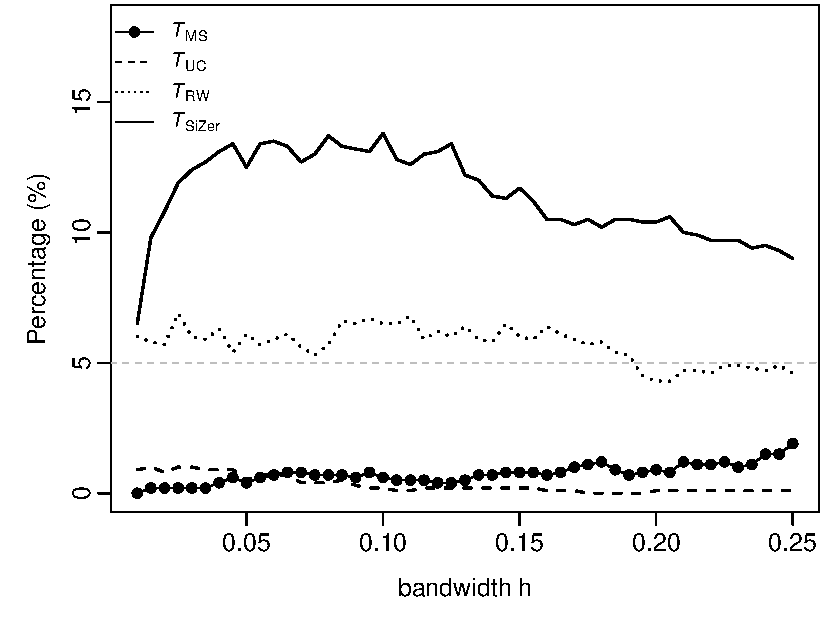
\includegraphics[width=\linewidth]{Plots/pcp_size_T_1000_a1_-50.pdf}
\caption{$a_1 = -0.5$}
\end{subfigure}
\begin{subfigure}{.5\textwidth}
\centering
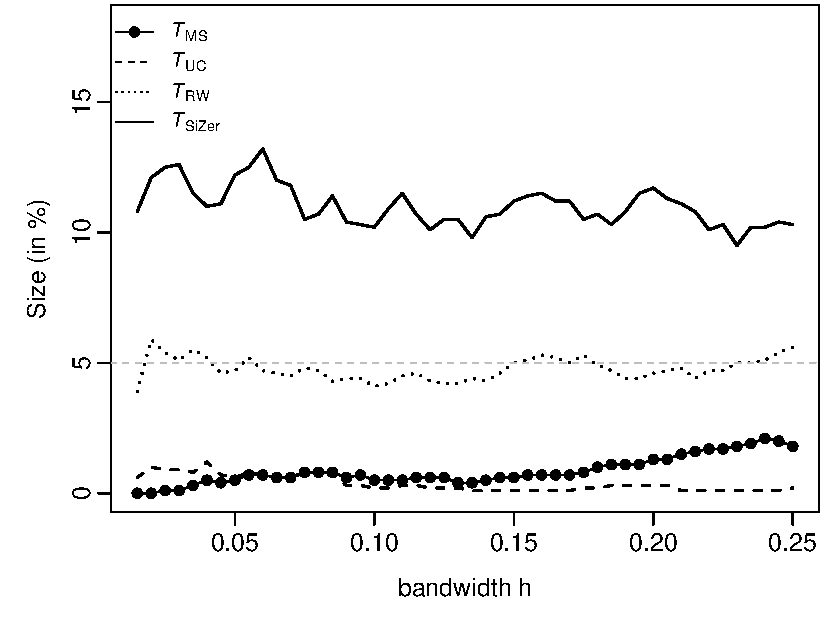
\includegraphics[width=\linewidth]{Plots/pcp_size_T_1000_a1_50.pdf}
\caption{$a_1 = 0.5$}
\end{subfigure}
\caption{Row-wise size comparisons for the significance level $\alpha=5\%$ and the sample size $T=1000$. Subfigure (a) corresponds to the case with $a_1=-0.5$, subfigure (b) to the case with $a_1=0.5$.}\label{fig:sim:size:compare}
\end{figure}


%We conduct some simulations to illustrate this distinction. The results are as expected: Our multiscale test $\mathcal{T}_{\text{MS}}$ and its uncorrected version $\mathcal{T}_{\text{UC}}$ hold the size $\alpha$ reasonably well, whereas the row-wise procedures $\mathcal{T}_{\text{RW}}$ and $\mathcal{T}_{\text{SiZer}}$ are much too liberal, their size lying substantially above the target $\alpha$. On the other hand, the row-wise procedures have good size properties when each scale $h \in H$ is considered separately.  As the result are not much insightful, we have not included them in the paper but we have added them to the Supplementary NMAteria in Section S.3. 


We conduct some simulation exercises to illustrate this important distinction. To keep the simulation study to a reasonable length, we restrict attention to the significance level $\alpha=0.05$ and the AR parameters $a_1 \in \{-0.5,0.5\}$. To simplify the implementation of $\mathcal{T}_{\text{SiZer}}$, we assume that the autocovariance function of the error process and thus the long-run error variance $\sigma^2$ is known. To keep the comparison fair, we treat $\sigma^2$ as known also when implementing $\mathcal{T}_{\text{MS}}$, $\mathcal{T}_{\text{UC}}$ and $\mathcal{T}_{\text{RW}}$. Moreover, we use exactly the same location-scale grid for all four methods. To achieve this, we start off with the grid $\mathcal{G}_T = U_T \times H_T$ with $U_T$ and $H_T$ defined above. We then follow \cite{Rondonotti2007} and \cite{ParkHannigKang2009} and restrict attention to those points $(u,h) \in \mathcal{G}_T$ for which the effective sample size $\text{ESS}^*(u,h)$ for correlated data is not smaller than $5$. This yields the grid $\mathcal{G}_T^* = \{ (u, h) \in \mathcal{G}_T : \text{ESS}^*(u, h) \geq 5 \}$. A definition of $\text{ESS}^*(u,h)$ is given in Section S.3 of the Supplement. 


In what follows, we distinguish between global and row-wise (or scale-wise) size: Global size is defined as the percentage of simulations in which the test under consideration rejects $H_0(u,h)$ for some $(u,h) \in \mathcal{G}_T^*$. Hence, it is identical to the size as computed in Tables \ref{tab:sim:size:MS1} and \ref{tab:sim:size:MS2}. Row-wise size for scale $h^* \in H_T$, in contrast, is the percentage of simulations in which the test rejects $H_0(u,h^*)$ for some $(u,h^*) \in \mathcal{G}_T^*$. %Hence, the size is calculated for each scale $h^*$ separately. 
Table \ref{tab:sim:size:compare} reports the global size of the four tests. As can be seen, the size of our multiscale test $\mathcal{T}_{\text{MS}}$ is fairly close to the target $\alpha=0.05$. The size numbers of the uncorrected version $\mathcal{T}_{\text{UC}}$ are reasonably close to $\alpha=0.05$ as well, even though they are a bit upward biased for $a_1=-0.5$ and downward biased for $a_1=0.5$. The global size of the row-wise methods $\mathcal{T}_{\text{RW}}$ and $\mathcal{T}_{\text{SiZer}}$, in contrast, is much larger than the target $\alpha=0.05$. Hence, as expected, the global tests $\mathcal{T}_{\text{MS}}$ and $\mathcal{T}_{\text{UC}}$ hold the size reasonably well, whereas the row-wise methods $\mathcal{T}_{\text{RW}}$ and $\mathcal{T}_{\text{SiZer}}$ are much too liberal. 


Figure \ref{fig:sim:size:compare} reports the row-wise size of the four tests by so-called parallel coordinate plots [\cite{Inselberg1985}] for the sample size $T=1000$. Each curve in the figure specifies the row-wise size of one of the tests for the scales $h$ under consideration. As can be seen, the row-wise version $\mathcal{T}_{\text{RW}}$ of our multiscale test holds the size quite accurately across scales. %Only for very fine scales, the size is not kept very precisely, which is presumably due to the fact that the effective sample size (i.e.\ the number of data points in the kernel window) is very small, leading to imprecise results. 
The row-wise size of $\mathcal{T}_{\text{SiZer}}$ also gives an acceptable approximation to the target $\alpha=5\%$, even though the size numbers are upward biased quite a bit. The global tests $\mathcal{T}_{\text{MS}}$ and $\mathcal{T}_{\text{UC}}$, in contrast, have a row-wise size much smaller than the target $\alpha=5\%$, which reflects the fact that they control global rather than row-wise size. 


\subsubsection{Power comparisons}\label{subsec-sim-multiscale-power}


In the second part of our simulation study, we compare the tests $\mathcal{T}_{\text{MS}}$, $\mathcal{T}_{\text{UC}}$, $\mathcal{T}_{\text{RW}}$ and $\mathcal{T}_{\text{SiZer}}$ in terms of power. As above, we use the location-scale grid $\mathcal{G}_T^*$ and treat the autocovariance function of the error terms as known when implementing the tests. Moreover, we restrict attention to the significance level $\alpha=0.05$, the AR parameters $a_1 \in \{-0.5,0.5\}$ and the sample size $T=1000$. Our simulation exercises investigate the ability of the four tests to detect local increases in the trend $m$. (The same could of course be done for decreases as well.) The tests indicate a local increase in $m$ according to the following decision rules: For each $(u,h) \in \mathcal{G}_T^*$, 
\begin{center}
\begin{tabular}{rcl}
$\mathcal{T}_{\text{MS}}$ indicates an increase on $[u-h,u+h]$   & $\Longleftrightarrow$ & $\widehat{\psi}_T(u,h) / \widehat{\sigma} > q_T(\alpha) + \lambda(h)$ \\ 
$\mathcal{T}_{\text{UC}}$ indicates an increase on $[u-h,u+h]$   & $\Longleftrightarrow$ & $\widehat{\psi}_T(u,h) / \widehat{\sigma} > q_T^{\text{UC}}(\alpha)$ \\
$\mathcal{T}_{\text{RW}}$ indicates an increase on $[u-h,u+h]$   & $\Longleftrightarrow$ & $\widehat{\psi}_T(u,h) / \widehat{\sigma} > q_T^{\text{RW}}(\alpha,h)$ \\
$\mathcal{T}_{\text{SiZer}}$ indicates an increase on $[u-h,u+h]$ & $\Longleftrightarrow$ & $s_T(u,h) > q_T^{\text{SiZer}}(\alpha,h)$, 
\end{tabular}
\end{center}
where $q_T^{\text{UC}}(\alpha)$, $q_T^{\text{RW}}(\alpha,h)$, $q_T^{\text{SiZer}}(\alpha,h)$ are the critical values of $\mathcal{T}_{\text{UC}}$, $\mathcal{T}_{\text{RW}}$, $\mathcal{T}_{\text{SiZer}}$, respectively. Note that the critical values of $\mathcal{T}_{\text{RW}}$ and $\mathcal{T}_{\text{SiZer}}$ depend on the scale $h$ as these are row-wise procedures. 


\begin{table}[t!]
\footnotesize{
\caption{Global power and global spurious power comparisons for $\alpha=0.05$ and $T=1000$.}\label{tab:sim:power:bump}
\newcolumntype{Z}{>{\centering\arraybackslash}X}
\begin{tabularx}{\textwidth}{l@{\hskip 20pt} Z@{\hskip 6pt}Z@{\hskip 6pt}Z@{\hskip 6pt}Z@{\hskip 20pt}Z@{\hskip 6pt}Z@{\hskip 6pt}Z@{\hskip 6pt}Z}
\toprule
 & \multicolumn{4}{c}{$a_1 = -0.5$} & \multicolumn{4}{c}{$a_1 = 0.5$} \\
\cmidrule[0.4pt]{2-9} 
 & $\mathcal{T}_{\text{MS}}$ & $\mathcal{T}_{\text{UC}}$ & $\mathcal{T}_{\text{RW}}$ & $\mathcal{T}_{\text{SiZer}}$ & $\mathcal{T}_{\text{MS}}$ & $\mathcal{T}_{\text{UC}}$ & $\mathcal{T}_{\text{RW}}$ & $\mathcal{T}_{\text{SiZer}}$ \\
\cmidrule[0.4pt]{1-9}
Global power           & 0.504 & 0.360 & 0.760 & 0.872  & 0.550 & 0.427 & 0.795 & 0.895 \\ 
Global spurious power  & 0.023 & 0.024 & 0.158 & 0.283  & 0.020 & 0.019 & 0.123 & 0.252 \\
\bottomrule
\end{tabularx}}
\vspace{0.2cm}
\end{table}


\begin{figure}[t!]
\begin{subfigure}{0.5\textwidth}
\centering
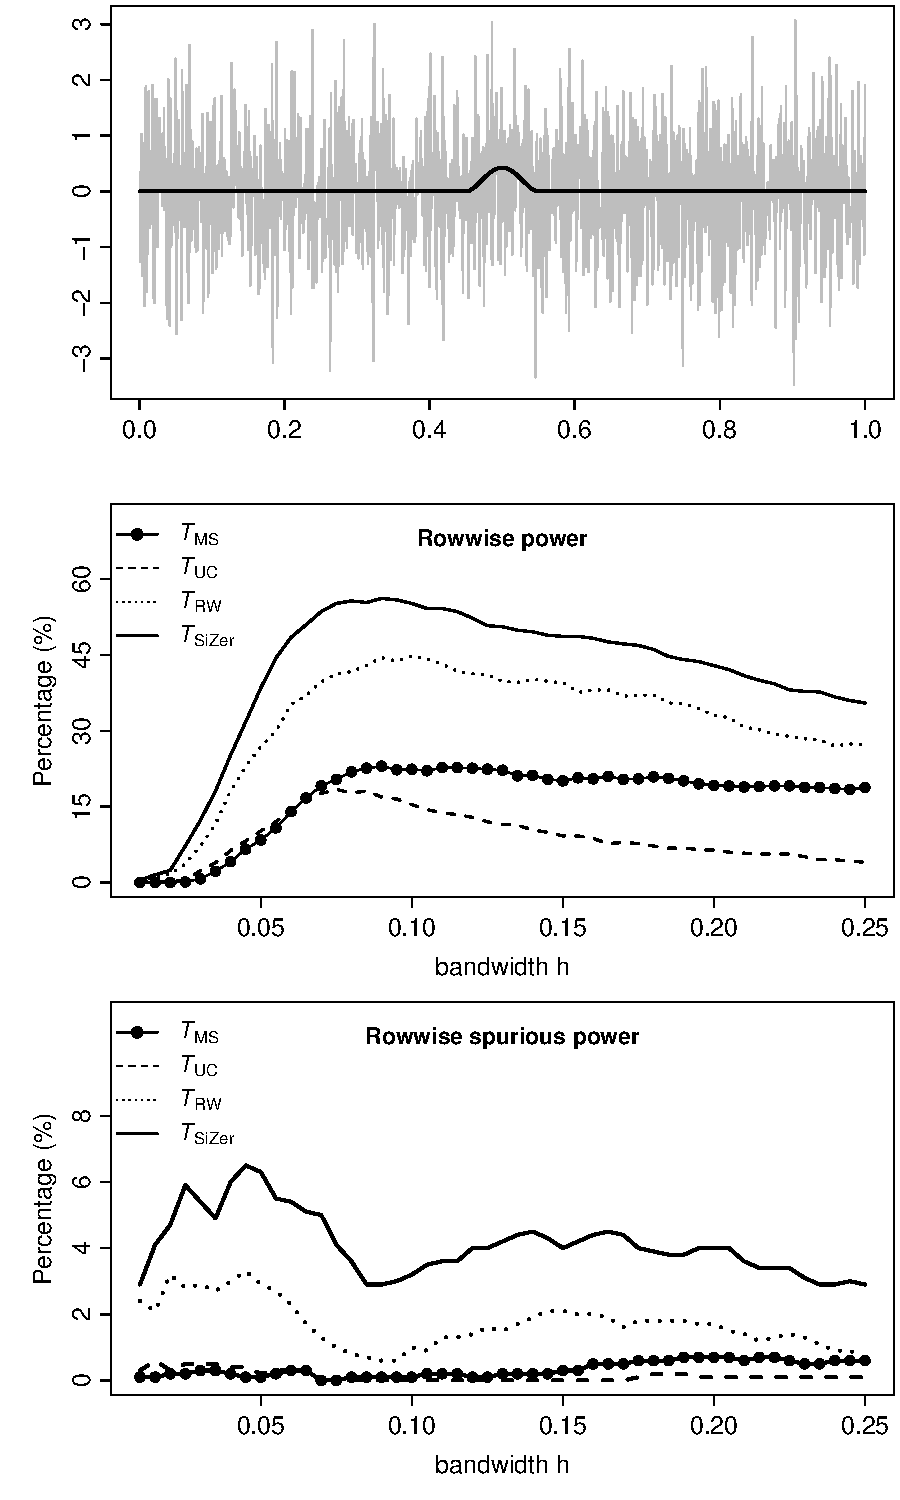
\includegraphics[width=\linewidth]{Plots/pcp_power_T_1000_a1_-50.pdf}
\caption{$a_1 = -0.5$}
\end{subfigure}
\begin{subfigure}{0.5\textwidth}
\centering
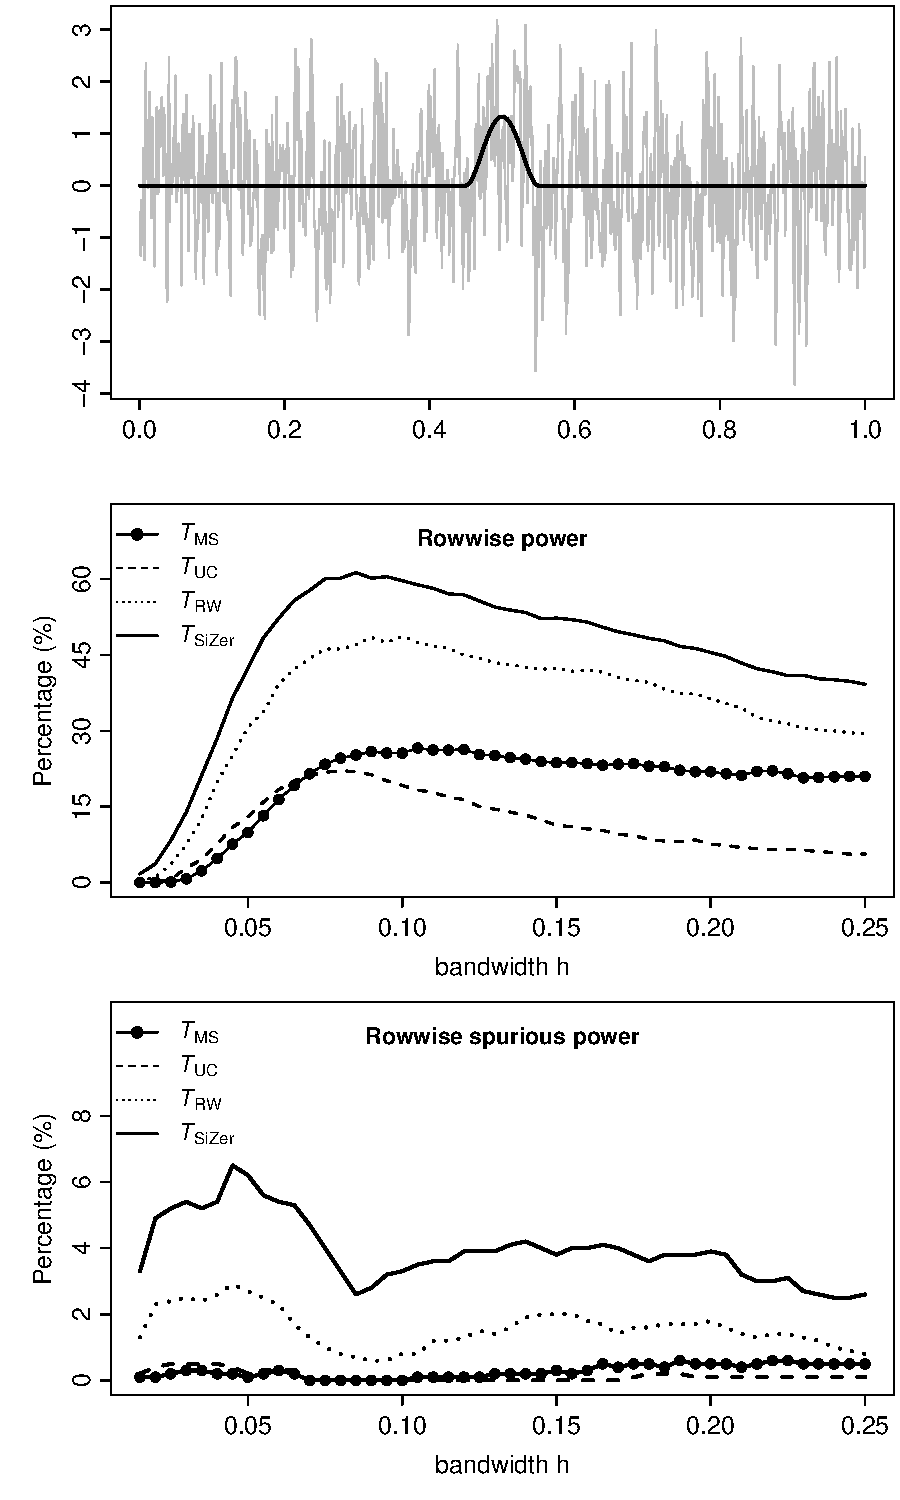
\includegraphics[width=\linewidth]{Plots/pcp_power_T_1000_a1_50.pdf}
\caption{$a_1 = 0.5$}
\end{subfigure}
\caption{Row-wise power and row-wise spurious power comparisons for $\alpha=5\%$ and $T=1000$. Subfigure (a) corresponds to the case with $a_1=-0.5$, subfigure (b) to the case with $a_1=0.5$. The upper panel of each subfigure shows the bump function $m$ with a representative data sample in the background. The parallel coordinate plot in the middle panel reports row-wise power, the plot in the lower panel reports row-wise spurious power.}\label{fig:sim:power:bump}
\end{figure}


To be able to make systematic power comparisons, we consider a very simple trend function $m$. More complicated signals $m$ are analyzed in Section ?? of the Supplementary Material. The trend function we are considering here is defined as $m(u) = c \cdot \ind(u \in [0.45,0.55]) \cdot (1 - \{\frac{(u-0.5}{0.05}\}^2)^2$, where $c = ??$ in the AR case with $a_1 = -0.5$ and $c=??$ in the case with $a_1=0.5$. The function $m$ is increasing on $I^{+} = (0.45,0.5)$, decreasing on $I^{-} = (0.5,0.55)$ and constant elsewhere. The two upper panels of Figure \ref{fig:sim:power:bump} give a graphical illustration of $m$, where the grey line in the background is the time series path of a representative simulated data sample. As can be seen, $m$ is a small bump around $u=0.5$, where $c$ determines the height of the bump. The constant $c$ is chosen such that the bump is difficult but not impossible to detect for the four tests. We distinguish between the following types of power for the tests $\mathcal{T}_j$ with $j \in \{ \text{MS}, \text{UC}, \text{RW}, \text{SiZer} \}$: 
\begin{enumerate}[label=(\roman*),leftmargin=0.85cm]
\item global power: the precentage of simulation runs in which the test $\mathcal{T}_j$ indicates an increase on some interval $I_{u,h}=[u-h,u+h]$ where $m$ is indeed increasing, that is, on some $I_{u,h}$ with $I_{u,h} \cap I^+ \neq \emptyset$.
\item spurious global power: the percentage of simulation runs in which the test $\mathcal{T}_j$ indicates an increase on some interval $I_{u,h}=[u-h,u+h]$ where $m$ is not increasing, that is, on some $I_{u,h}$ with $I_{u,h} \cap I^+ = \emptyset$.
\item row-wise power on scale $h^*$: the percentage of simulation runs in which the test $\mathcal{T}_j$ indicates an increase on some interval $I_{u,h^*}=[u-h^*,u+h^*]$ where $m$ is indeed increasing, that is, on some $I_{u,h^*}$ with $I_{u,h^*} \cap I^+ \neq \emptyset$.
\item spurious row-wise power on scale $h^*$: the percentage of simulation runs in which the test $\mathcal{T}_j$ indicates an increase on some interval $I_{u,h^*}=[u-h^*,u+h^*]$ where $m$ is not increasing, that is, on some $I_{u,h^*}$ with $I_{u,h^*} \cap I^+ = \emptyset$.
\end{enumerate}


Table \ref{tab:sim:power:bump} reports the global power and global spurious power of the four tests. As one can see, our multiscale test $\mathcal{T}_{\text{MS}}$ has higher power than the uncorrected version $\mathcal{T}_{\text{UC}}$. This confirms the theoretical optimality theory in \cite{DuembgenSpokoiny2001} [see also \cite{DuembgenWalther2008} and \cite{RufibachWalther2010}] according to which the aggregation scheme of $\mathcal{T}_{\text{MS}}$ should yield better power properties than the simpler scheme of $\mathcal{T}_{\text{UC}}$. As expected, the row-wise methods $\mathcal{T}_{\text{RW}}$ and $\mathcal{T}_{\text{SiZer}}$ have substantially more power than the global tests. Indeed, $\mathcal{T}_{\text{SiZer}}$ is even a bit more powerful than $\mathcal{T}_{\text{RW}}$, which is presumably due to the fact that it is a bit too liberal under the null as observed in Figure \ref{fig:sim:size:compare}. The higher power of the row-wise procedures comes at some cost: Their spurious global power is much higher than that of the global tests. In the case with $a_1=-0.5$, $\mathcal{T}_{\text{SiZer}}$ spuriously finds an increase in the trend $m$ in more than 28\% of the simulations, $\mathcal{T}_{\text{RW}}$ in more than $15\%$. The numbers for the case with $a_1=0.5$ are similar. The multiscale test $\mathcal{T}_{\text{MS}}$ (as well as its uncorrected version $\mathcal{T}_{\text{UC}}$), in contrast, controls the probability of finding a spurious increase. In particular, as implied by Proposition \ref{prop-test-3}, its spurious global power is below $100\cdot\alpha\% = 5\%$.  


Figure \ref{fig:sim:power:bump} gives a more detailed picture of the power properties of the four tests. The parallel coordinate plots of the figure show how power and spurious power are distributed across scales $h$. Let us first have a look at the row-wise methods. As can be seen, $\mathcal{T}_{\text{SiZer}}$ is more powerful than $\mathcal{T}_{\text{RW}}$ on all scales under consideration. As already mentioned when discussing the global power results, this is presumably due to the fact that $\mathcal{T}_{\text{SiZer}}$ is somewhat too liberal under the null. Comparing the power curves of the two global methods gives an interesting insight: Our multiscale test $\mathcal{T}_{\text{MS}}$ has substantially more power than the uncorrected version $\mathcal{T}_{\text{UC}}$ on medium and large scales. On small scales, in contrast, it is slightly less powerful than $\mathcal{T}_{\text{UC}}$. This again illustrates the theoretical optimality theory in \cite{DuembgenSpokoiny2001} which suggests that, asymptotically, the multiscale test $\mathcal{T}_{\text{MS}}$ should be as powerful as $\mathcal{T}_{\text{UC}}$ on small scales but more powerful on large scales. This is essentially what we see in the two middle panels of Figure \ref{fig:sim:power:bump}. Of course, $\mathcal{T}_{\text{MS}}$ does not have exactly as much power as $\mathcal{T}_{\text{UC}}$ on fine scales. However, the loss of power on fine scales is very small compared to the gain of power on larger scales (which is also reflected by the fact that $\mathcal{T}_{\text{MS}}$ has more global power than $\mathcal{T}_{\text{UC}}$). 


The main take-aways from our simulation exercises are as follows: If one is interested in an exploratory data tool for finding local increases/decreases of a trend, the row-wise methods $\mathcal{T}_{\text{RW}}$ and $\mathcal{T}_{\text{SiZer}}$ both do a good job. However, if one wants to make rigorous statistical inference, in particular, rigorous confidence statements about local increases/decreases of the trend, one needs to go for a global test method. Our simulation exercises have demonstrated that our multiscale test $\mathcal{T}_{\text{MS}}$ is a global method which enjoys good size and power properties. In particular, as predicted by the theory, it is a more effective test than the uncorrected version $\mathcal{T}_{\text{UC}}$. 


\subsection{Small sample properties of the long-run variance estimator}\label{subsec-sim-lrv}


\textcolor{red}{In the final part of our simulation study, we analyze the estimators of the AR parameters and the long-run error variance from Section \ref{sec-error-var} and compare them to the estimators of \cite{Hall2003}. We simulate data from the model $Y_{t,T} = m(t/T) + \varepsilon_t$, where $\{ \varepsilon_t\}$ is an AR($1$) process of the form $\varepsilon_t = a_1 \varepsilon_{t-1} + \eta_t$. We consider the AR parameters $a_1 \in \{-0.95,-0.75,-0.5,-0.25,0.25,0.5,0.75,0.95\}$ and let $\eta_t$ be i.i.d.\ standard normal innovation terms. Throughout the simulation study, the AR order $p^*=1$ is treated as known.} We report our findings for a specific sample size $T$, in particular for $T=500$, as the results for other sample sizes are very similar. For simplicity, $m$ is chosen to be a linear function of the form $m(u) = \beta u$ with the slope parameter $\beta$. For each value of $a_1$, we consider two different slopes $\beta$, one corresponding to a moderate and one to a pronounced trend $m$. 
%In particular, we let $\beta = s_\beta \cdot \sigma$ with $s_\beta = 1$ (moderate trend) and $s_\beta= 10$ (pronounced trend), where $\sigma^2$ is the long-run error variance.
In particular, we let $\beta = s_\beta \sqrt{\var(\varepsilon_t)}$ with $s_\beta \in \{1,10\}$. When $s_\beta = 1$, the slope $\beta$ is equal to the standard deviation $\sqrt{\var(\varepsilon_t)}$ of the error process, which yields a moderate trend $m$. When $s_\beta = 10$, in contrast, the slope $\beta$ is $10$ times as large as $\sqrt{\var(\varepsilon_t)}$, which results in a quite pronounced trend $m$. 


For each model specification, we generate $S=1000$ data samples and compute the following quantities for each simulated sample: 
\begin{enumerate}[label=(\roman*),leftmargin=0.9cm]
\item the pilot estimator $\widetilde{a}_q$ from \eqref{est-AR-FS} with the tuning parameter $q$.
\item the estimator $\widehat{a}$ from \eqref{est-AR} with the tuning parameter $\overline{r}$ as well as the long-run variance estimator $\widehat{\sigma}^2$ from \eqref{est-lrv}. 
\item the estimators of $a_1$ and $\sigma^2$ from \cite{Hall2003}, which are denoted by $\widehat{a}_{\text{HvK}}$ and $\widehat{\sigma}^2_{\text{HvK}}$ for ease of reference. The estimator $\widehat{a}_{\text{HvK}}$ is computed as described in Section 2.2 of \cite{Hall2003} and $\widehat{\sigma}^2_{\text{HvK}}$ as defined at the bottom of p.447 in Section 2.3. The estimator $\widehat{a}_{\text{HvK}}$ (as well as $\widehat{\sigma}^2_{\text{HvK}}$) depends on two tuning parameters which we denote by $m_1$ and $m_2$ as in \cite{Hall2003}. 
\item oracle estimators $\widehat{a}_{\text{oracle}}$ and $\widehat{\sigma}^2_{\text{oracle}}$ of $a_1$ and $\sigma^2$, which are constructed under the assumption that the error process $\{\varepsilon_t\}$ is observed. For each simulation run, we compute $\widehat{a}_{\text{oracle}}$ as the maximum likelihood estimator of $a_1$ from the time series of simulated error terms $\varepsilon_1,\ldots,\varepsilon_T$. We then calculate the residuals $r_t = \varepsilon_t - \widehat{a}_{\text{oracle}} \, \varepsilon_{t-1}$ and estimate the innovation variance $\nu^2 = \ex[\eta_t^2]$ by $\widehat{\nu}_{\text{oracle}}^2 = (T-1)^{-1} \sum_{t=2}^T r_t^2$. Finally, we set $\widehat{\sigma}^2_{\text{oracle}} = \widehat{\nu}_{\text{oracle}}^2 / (1 - \widehat{a}_{\text{oracle}})^2$. 
\end{enumerate}
Throughout the section, we set $q = 25$, $\overline{r} = 10$ and $(m_1,m_2) = (20,30)$. We in particular choose $q$ to be in the middle of $m_1$ and $m_2$ to make the tuning parameters of the estimators $\widetilde{a}_q$ and $\widehat{a}_{\text{HvK}}$ more or less comparable. In order to assess how sensitive our estimators are to the choice of $q$ and $\overline{r}$, we carry out a number of robustness checks, considering a range of different values for $q$ and $\overline{r}$. In addition, we vary the tuning parameters $m_1$ and $m_2$ of the estimators from \cite{Hall2003} in order to make sure that the results of our comparison study are not driven by the particular choice of any of the involved tuning parameters. The results of our robustness checks are reported in Section S.3 of the Supplementary Material. They show that the results of our comparison study are robust to %persist across 
different choices of the parameters $q$, $\overline{r}$ and $(m_1,m_2)$. %Moreover, they indicate that our estimators are rather insensitive to the choice of tuning parameters. 


\begin{figure}[t!]
\begin{subfigure}[b]{0.475\textwidth}
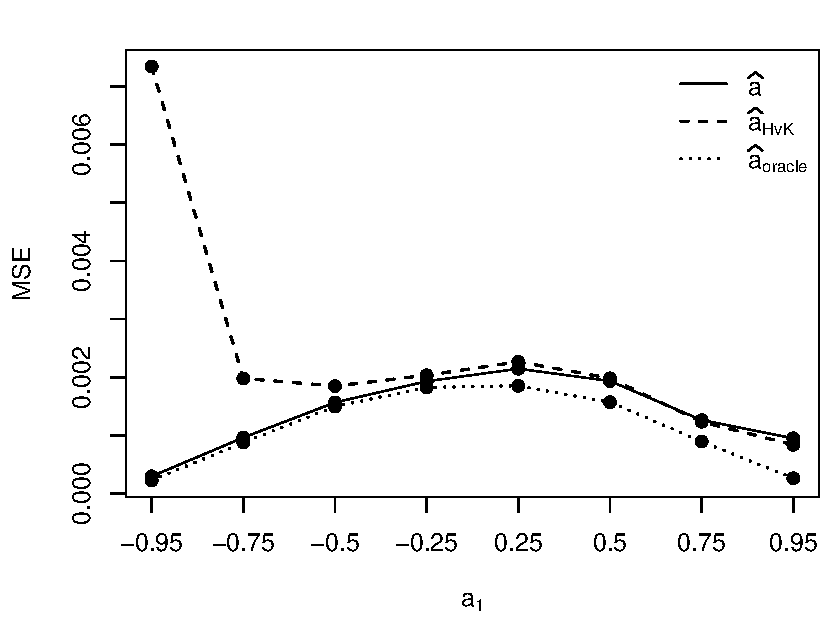
\includegraphics[width=\textwidth]{Plots/MSE_a1_T=500_slope=1_(q,r,M1,M2)=(25,10,20,30).pdf}
\end{subfigure}\hspace{0.25cm}
\begin{subfigure}[b]{0.475\textwidth}
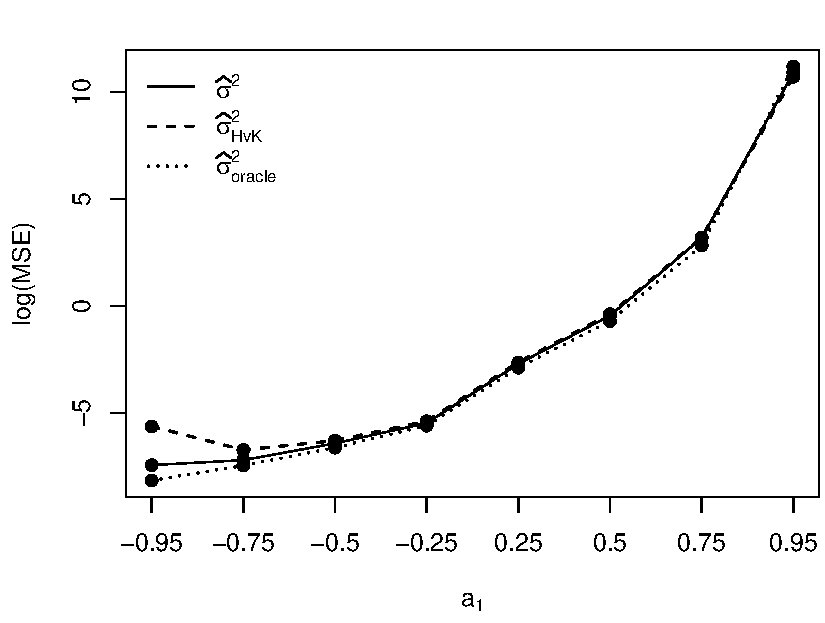
\includegraphics[width=\textwidth]{Plots/MSE_lrv_T=500_slope=1_(q,r,M1,M2)=(25,10,20,30).pdf}
\end{subfigure}
\caption{MSE values for the estimators $\widehat{a}$, $\widehat{a}_{\text{HvK}}$, $\widehat{a}_{\text{oracle}}$ and $\widehat{\sigma}^2$, $\widehat{\sigma}^2_{\text{HvK}}$, $\widehat{\sigma}^2_{\text{oracle}}$ in the simulation scenarios with a moderate trend ($s_\beta=1$).}\label{fig:MSE_slope1}
%\end{figure}
\vspace{0.25cm}


%\begin{figure}[t!]
\begin{subfigure}[b]{0.475\textwidth}
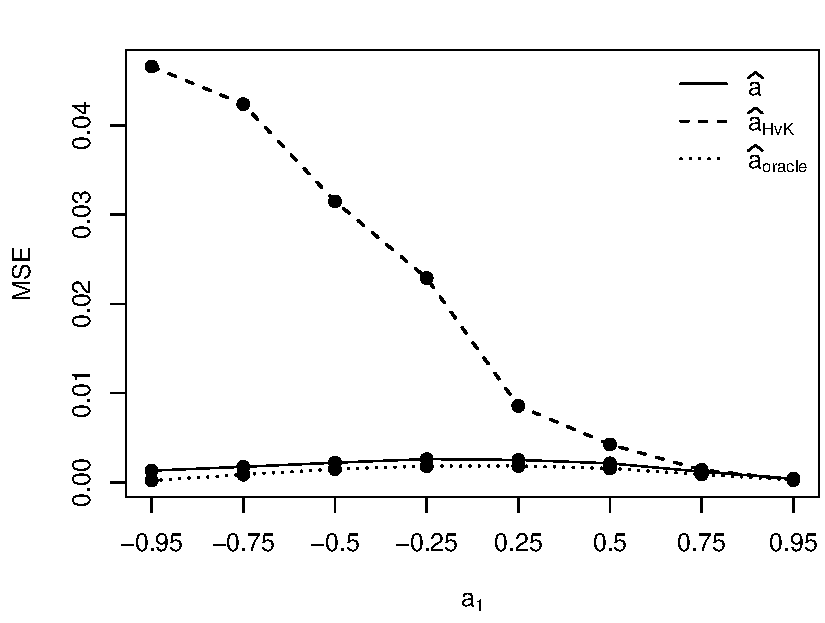
\includegraphics[width=\textwidth]{Plots/MSE_a1_T=500_slope=10_(q,r,M1,M2)=(25,10,20,30).pdf}
\end{subfigure}\hspace{0.25cm}
\begin{subfigure}[b]{0.475\textwidth}
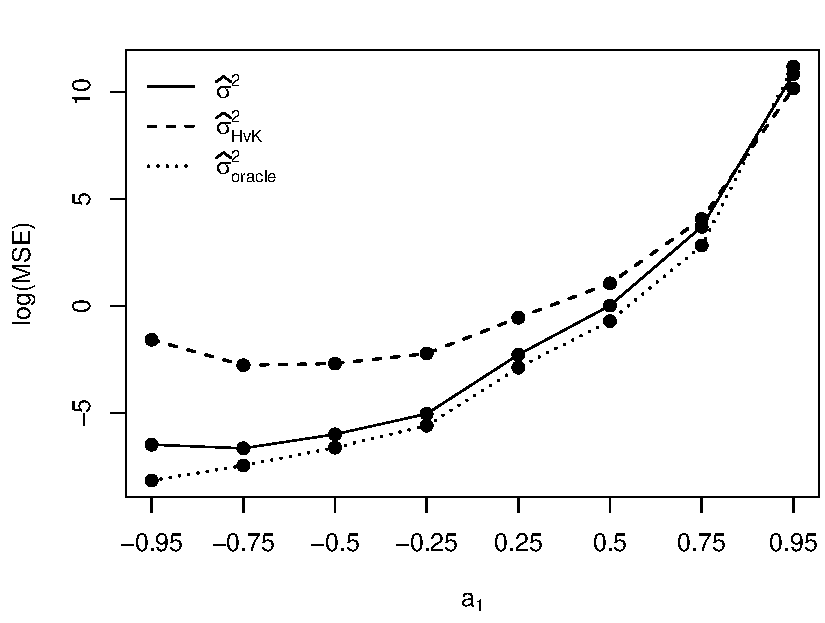
\includegraphics[width=\textwidth]{Plots/MSE_lrv_T=500_slope=10_(q,r,M1,M2)=(25,10,20,30).pdf}
\end{subfigure}
\caption{MSE values for the estimators $\widehat{a}$, $\widehat{a}_{\text{HvK}}$, $\widehat{a}_{\text{oracle}}$ and $\widehat{\sigma}^2$, $\widehat{\sigma}^2_{\text{HvK}}$, $\widehat{\sigma}^2_{\text{oracle}}$ in the simulation scenarios with a pronounced trend ($s_\beta=10$).}\label{fig:MSE_slope10}
\end{figure}


\begin{figure}[t!]
\centering
\begin{subfigure}[b]{\textwidth}
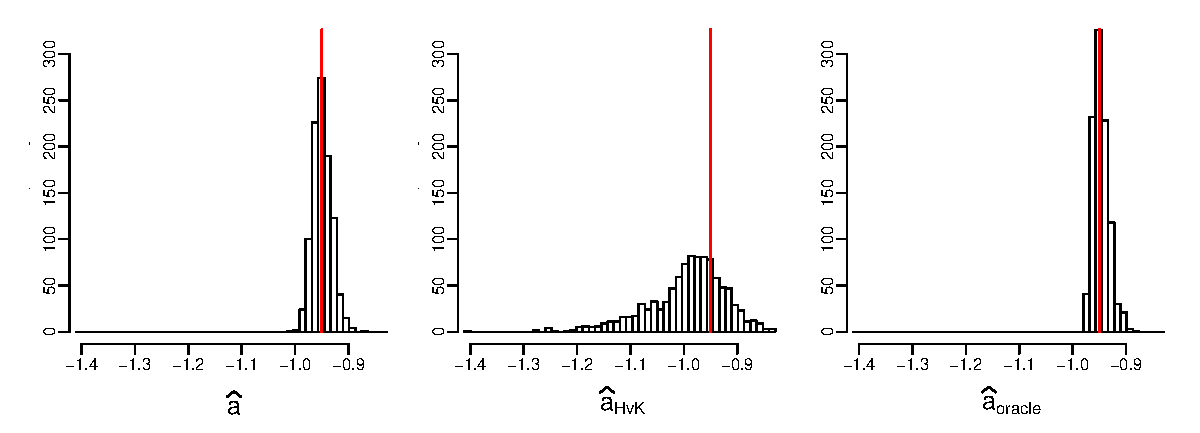
\includegraphics[width=\textwidth]{Plots/a_hat_histograms_a1=-95_T=500_slope=1_(q,r,M1,M2)=(25,10,20,30).pdf}
\end{subfigure}
\begin{subfigure}[b]{\textwidth}
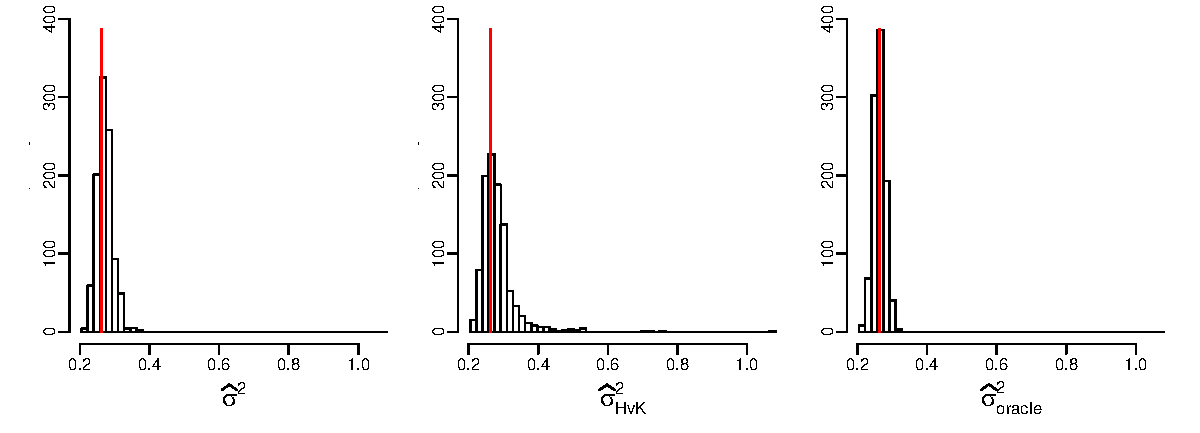
\includegraphics[width=\textwidth]{Plots/lrv_histograms_a1=-95_T=500_slope=1_(q,r,M1,M2)=(25,10,20,30).pdf}
\end{subfigure}
\caption{Histograms of the simulated values produced by the estimators $\widehat{a}$, $\widehat{a}_{\text{HvK}}$, $\widehat{a}_{\text{oracle}}$ and $\widehat{\sigma}^2$, $\widehat{\sigma}^2_{\text{HvK}}$, $\widehat{\sigma}^2_{\text{oracle}}$ in the scenario with $a_1 = -0.95$ and $s_\beta = 1$. The vertical red lines indicate the true values of $a_1$ and $\sigma^2$.}\label{fig:hist_scenario1} 
\end{figure}


\begin{figure}[t!]
\centering
\begin{subfigure}[b]{\textwidth}
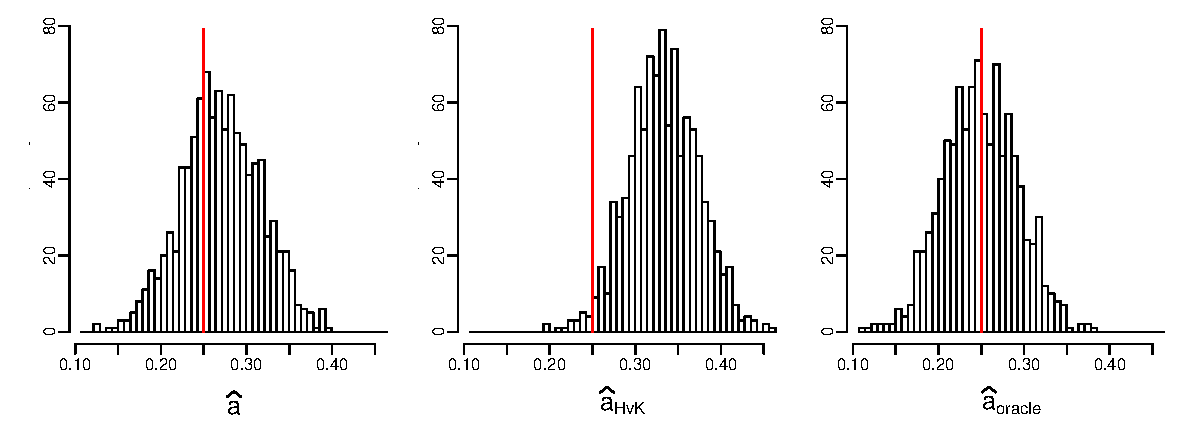
\includegraphics[width=\textwidth]{Plots/a_hat_histograms_a1=25_T=500_slope=10_(q,r,M1,M2)=(25,10,20,30).pdf}
\end{subfigure}
\begin{subfigure}[b]{\textwidth}
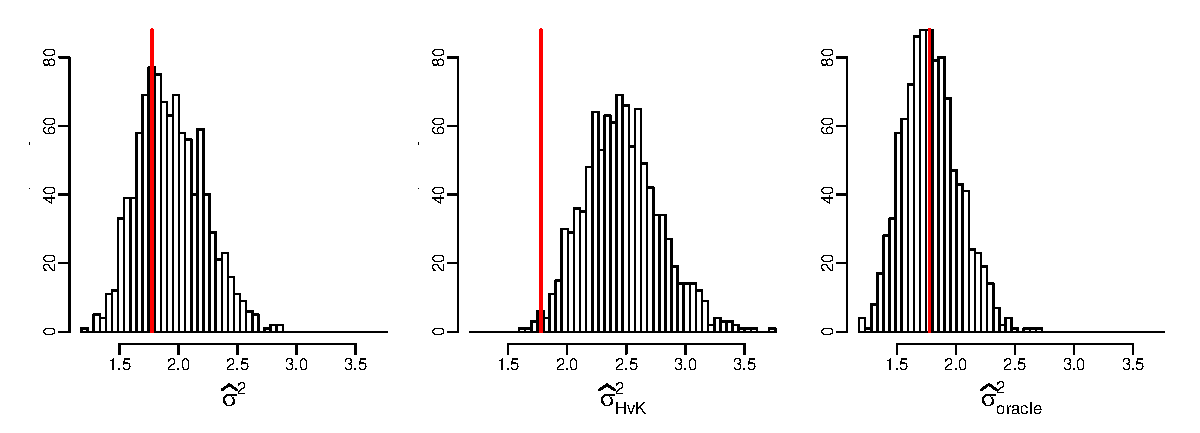
\includegraphics[width=\textwidth]{Plots/lrv_histograms_a1=25_T=500_slope=10_(q,r,M1,M2)=(25,10,20,30).pdf}
\end{subfigure}
\caption{Histograms of the simulated values produced by the estimators $\widehat{a}$, $\widehat{a}_{\text{HvK}}$, $\widehat{a}_{\text{oracle}}$ and $\widehat{\sigma}^2$, $\widehat{\sigma}^2_{\text{HvK}}$, $\widehat{\sigma}^2_{\text{oracle}}$ in the scenario with $a_1 = 0.25$ and $s_\beta = 10$. The vertical red lines indicate the true values of $a_1$ and $\sigma^2$.}\label{fig:hist_scenario2} 
\end{figure}


For each estimator $\widehat{a}$, $\widehat{a}_{\text{HvK}}$, $\widehat{a}_{\text{oracle}}$ and $\widehat{\sigma}^2$, $\widehat{\sigma}^2_{\text{HvK}}$, $\widehat{\sigma}^2_{\text{oracle}}$ and for each model specification, the simulation output consists in a vector of length $S=1000$ which contains the $1000$ simulated values of the respective estimator. Figures \ref{fig:MSE_slope1} and \ref{fig:MSE_slope10} report the mean squared error (MSE) of these $1000$ simulated values for each estimator. On the $x$-axis of each plot, the various values of the AR parameter $a_1$ are listed which are considered. The solid line in each plot gives the MSE values of our estimators. The dashed and dotted lines specify the MSE values of the HvK and the oracle estimators, respectively. Note that for the long-run variance estimators, the plots report the logarithm of the MSE rather than the MSE itself since the MSE values are too different across simulation scenarios to obtain a reasonable graphical presentation. In addition to the MSE values presented in Figures \ref{fig:MSE_slope1} and \ref{fig:MSE_slope10}, we depict histograms of the $1000$ simulated values produced by the estimators $\widehat{a}$, $\widehat{a}_{\text{HvK}}$, $\widehat{a}_{\text{oracle}}$ and $\widehat{\sigma}^2$, $\widehat{\sigma}^2_{\text{HvK}}$, $\widehat{\sigma}^2_{\text{oracle}}$ for two specific simulation scenarios in Figures \ref{fig:hist_scenario1} and \ref{fig:hist_scenario2}. The main findings can be summarized as follows:  
\begin{enumerate}[label=(\alph*),leftmargin=0.7cm]

%\item The performance of our second-step estimators $\widehat{a}$ and $\widehat{\sigma}^2$ is fairly close to that of the oracle estimators $\widehat{a}_{\text{oracle}}$ and $\widehat{\sigma}^2_{\text{oracle}}$ in all of the considered simulation scenarios. In particular, the mean values and standard deviations in Tables \ref{tab:AR_parameters} and \ref{tab:lrv} are quite similar for our estimators and the corresponding oracles. 

\item In the simulation scenarios with a moderate trend ($s_\beta = 1$), the estimators $\widehat{a}_{\text{HvK}}$ and $\widehat{\sigma}^2_{\text{HvK}}$ of \cite{Hall2003} exhibit a similar performance as our estimators $\widehat{a}$ and $\widehat{\sigma}^2$ as long as the AR parameter $a_1$ is not too close to $-1$. For strongly negative values of $a_1$ (in particular for $a_1 = -0.75$ and $a_1 = -0.95$), the estimators perform much worse than ours. This can be clearly seen from the much larger MSE values of the estimators  $\widehat{a}_{\text{HvK}}$ and $\widehat{\sigma}^2_{\text{HvK}}$ for $a_1 = -0.75$ and $a_1 = -0.95$ in Figure \ref{fig:MSE_slope1}. Figure \ref{fig:hist_scenario1} gives some further insights into what is happening here. It shows the histograms of the simulated values produced by the estimators $\widehat{a}$, $\widehat{a}_{\text{HvK}}$, $\widehat{a}_{\text{oracle}}$ and the corresponding long-run variance estimators in the scenario with $a_1=-0.95$ and $s_\beta = 1$. As can be seen, the estimator $\widehat{a}_{\text{HvK}}$ does not obey the causality restriction $|a_1| \le 1$ but frequently takes values substantially smaller than $-1$. This results in a very large spread of the histogram and thus in a disastrous performance of the estimator.\footnote{One could of course set $\widehat{a}_{\text{HvK}}$ to $-(1 - \delta)$ for some small $\delta > 0$ whenever it takes a value smaller than $-1$. This modified estimator, however, is still far from performing in a satisfying way when $a_1$ is close to $-1$.} A similar point applies to the histogram of the long-run variance estimator $\widehat{\sigma}^2_{\text{HvK}}$. Our estimators $\widehat{a}$ and $\widehat{\sigma}^2$, in contrast, exhibit a stable behaviour in this case. \\ %An analogous point applies to the long-run variance estimators $\widehat{\sigma}^2$ and $\widehat{\sigma}^2_{\text{HvK}}$. 
Interestingly, the estimator $\widehat{a}_{\text{HvK}}$ (as well as the corresponding long-run variance estimator $\widehat{\sigma}^2_{\text{HvK}}$) performs much worse than ours for large negative values but not for large positive values of $a_1$. This can be explained as follows: In the special case of an AR($1$) process, the estimator $\widehat{a}_{\text{HvK}}$ may produce estimates smaller than $-1$ but it cannot become larger than $1$. This can be easily seen upon inspecting the definition of the estimator. Hence, for large positive values of $a_1$, the estimator $\widehat{a}_{\text{HvK}}$ performs well as it satisfies the causality restriction that the estimated AR parameter should be smaller than $1$. 

\item In the simulation scenarios with a pronounced trend ($s_\beta = 10$), the estimators of \cite{Hall2003} are clearly outperformed by ours for most of the AR parameters $a_1$ under consideration. In particular, their MSE values reported in Figure \ref{fig:MSE_slope10} are much larger than the values produced by our estimators for most parameter values $a_1$. The reason is the following: The HvK estimators have a strong bias since the pronounced trend with $s_\beta = 10$ is not eliminated appropriately by the underlying differencing methods. This point is illustrated by Figure \ref{fig:hist_scenario2} which shows histograms of the simulated values for the estimators $\widehat{a}$, $\widehat{a}_{\text{HvK}}$, $\widehat{a}_{\text{oracle}}$ and the corresponding long-run variance estimators in the scenario with $a_1=0.25$ and $s_\beta = 10$. As can be seen, the histogram produced by our estimator $\widehat{a}$ is approximately centred around the true value $a_1 = 0.25$, whereas that of the estimator $\widehat{a}_{\text{HvK}}$ is strongly biased upwards. A similar picture arises for the long-run variance estimators $\widehat{\sigma}^2$ and $\widehat{\sigma}^2_{\text{HvK}}$. \\
Whereas the methods of \cite{Hall2003} perform much worse than ours for negative and moderately positive values of $a_1$, the performance (in terms of MSE) is fairly similar for large values of $a_1$. This can be explained as follows: When the trend $m$ is not eliminated appropriately by taking differences, this creates spurious persistence in the data. Hence, the estimator $\widehat{a}_{\text{HvK}}$ tends to overestimate the AR parameter $a_1$, that is, $\widehat{a}_{\text{HvK}}$ tends to be larger in absolute value than $a_1$. Very loosely speaking, when the parameter $a_1$ is close to $1$, say $a_1 = 0.95$, there is not much room for overestimation since $\widehat{a}_{\text{HvK}}$ cannot become larger than $1$. Consequently, the effect of not eliminating the trend appropriately has a much smaller impact on $\widehat{a}_{\text{HvK}}$ for large positive values of $a_1$. 

%\item In all of the simulation scenarios under consideration, in particular both when the trend is moderate ($s_\beta = 1$) and pronounced ($s_\beta = 10$), the MSE values produced by our estimators are fairly close to those of the oracle estimators as can be seen by inspecting Figures \ref{fig:MSE_slope1} and \ref{fig:MSE_slope10}. Only  

\end{enumerate}



\section{Application}\label{sec-data}


The analysis of time trends in long temperature records is an important task in climatology. Information on the shape of the trend is needed in order to better understand long-term climate variability. The Central England temperature record is the longest instrumental temperature time series in the world. It is a valuable asset for analysing climate variability over the last few hundred years. The data is publicly available on the webpage of the UK Met Office. A detailed description of the data can be found in \cite{Parker1992}. For our analysis, we use the dataset of yearly mean temperatures which consists of $T=359$ observations covering the years from $1659$ to $2017$. 


We assume that the data follow the nonparametric trend model $Y_{t,T} = m(t/T) + \varepsilon_t$, where $m$ is the unknown time trend of interest. The error process $\{ \varepsilon_t \}$ is supposed to have the AR($p$) structure $\varepsilon_t = \sum_{j=1}^p a_j \varepsilon_{t-j} + \eta_t$, where $\eta_t$ are i.i.d.\ innovations with mean $0$ and variance $\nu^2$. As pointed out in \cite{Mudelsee2010} among others, this is the most widely used error model for discrete climate time series. To select the AR order $p$, we proceed as follows: We estimate the AR parameters and the corresponding variance of the innovation terms for different AR orders by our methods from Section \ref{subsec-error-var-AR} and choose $p$ to be the minimizer of the Bayesian information criterion (BIC). This yields the AR order $p = 2$. We then estimate the parameters $\boldsymbol{a} = (a_1,a_2)$ and the long-run error variance $\sigma^2$ by the estimators $\widehat{\boldsymbol{a}} = (\widehat{a}_1,\widehat{a}_2)$ and $\widehat{\sigma}^2$, which gives the values  $\widehat{a}_1 = 0.167$, $\widehat{a}_2 = 0.178$ and $\widehat{\sigma}^2 = 0.749$. To select the AR order $p$ and to produce the estimators $\widehat{\boldsymbol{a}}$ and $\widehat{\sigma}^2$, we set $q = 25$ and $\overline{r} = 10$ as in the simulation study of Section \ref{subsec-sim-1}.\footnote{As a robustness check, we have repeated the process of order selection and parameter estimation for other values of $q$ and $\overline{r}$ as well as for other criteria such as FPE, AIC and AICC, which gave similar results.} 


\begin{figure}[t]
\centering
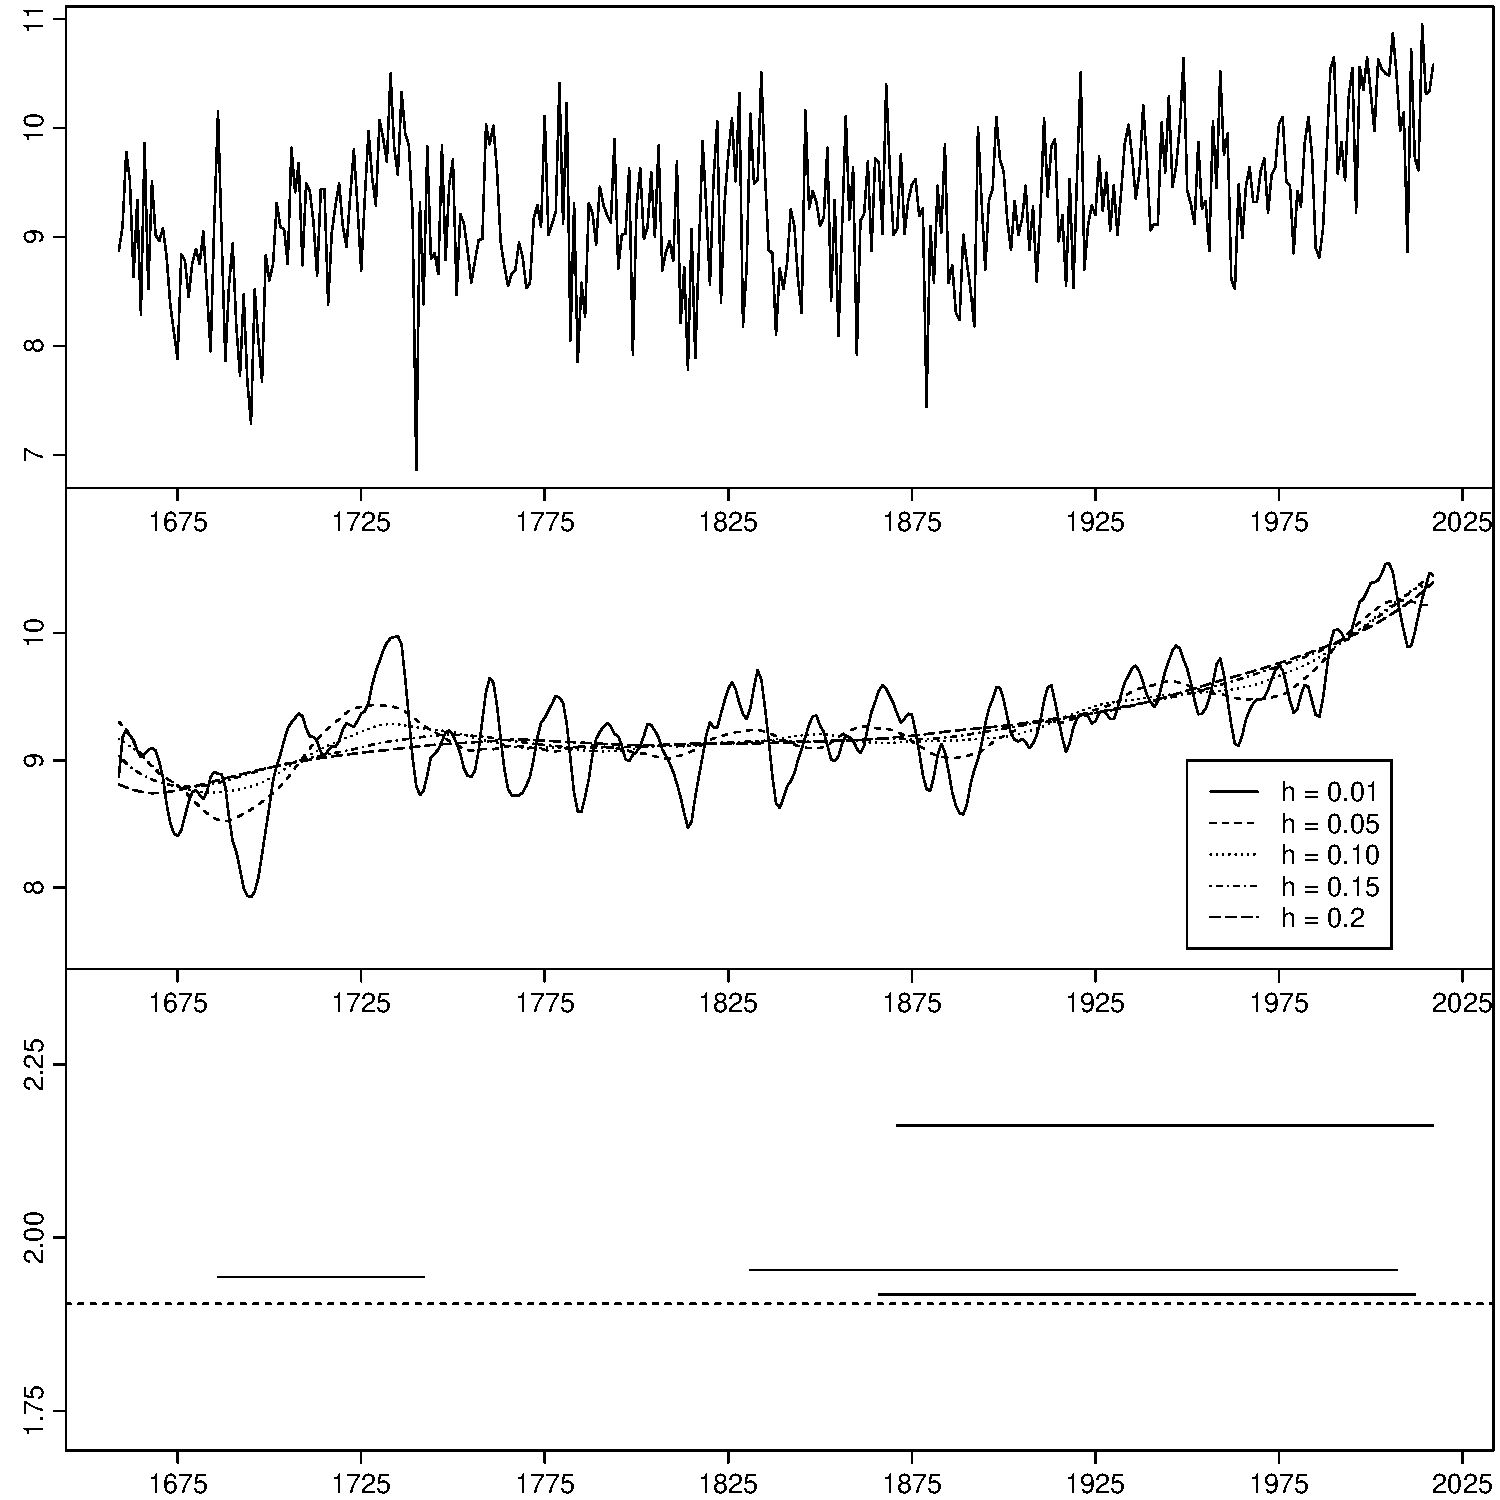
\includegraphics[width=0.8\textwidth]{Plots/temperature_data.pdf}
\caption{Summary of the application results. The upper panel shows the Central England mean temperature time series. The middle panel depicts local linear kernel estimates of the time trend for a number of different bandwidths $h$. The lower panel presents the minimal intervals in the set $\Pi_T^+$ produced by the multiscale test. These are $[1686,1742]$, $[1831,2007]$, $[1866, 2012]$ and $[1871,2017]$.}\label{plot-results-app1}
\end{figure}


With the help of our multiscale method from Section \ref{sec-method}, we now test the null hypothesis $H_0$ that $m$ is constant on all intervals $[u-h,u+h]$ with $(u,h) \in \mathcal{G}_T$, where we use the grid $\mathcal{G}_T$ defined in \eqref{grid-sim-app}. To do so, we set the significance level to $\alpha = 0.05$ and implement the test in exactly the same way as in the simulations of Section \ref{subsec-sim-1}. The results are presented in Figure \ref{plot-results-app1}. The upper panel shows the raw temperature time series, whereas the middle panel depicts local linear kernel estimates of the trend $m$ for different bandwidths $h$. As one can see, the shape of the estimated time trend strongly differs with the chosen bandwidth. When the bandwidth is small, there are many local increases and decreases in the estimated trend. When the bandwidth is large, most of these local variations get smoothed out. Hence, by themselves, the nonparametric fits do not give much information on whether the trend $m$ is increasing or decreasing in certain time regions. 


Our multiscale test provides this kind of information, which is summarized in the lower panel of Figure \ref{plot-results-app1}. The plot depicts the minimal intervals contained in the set $\Pi_T^+$, which is defined in Section \ref{subsec-method-theo}. The set of intervals $\Pi_T^-$ is empty in the present case. The height at which a minimal interval $I_{u,h} = [u-h,u+h] \in \Pi_T^+$ is plotted indicates the value of the corresponding (additively corrected) test statistic $\widehat{\psi}_T(u,h) / \widehat{\sigma} - \lambda(h)$. The dashed line specifies the critical value $q_T(\alpha)$, where $\alpha = 0.05$ as already mentioned above. According to Proposition \ref{prop-test-3}, we can make the following simultaneous confidence statement about the collection of minimal intervals in $\Pi_T^+$. We can claim, with confidence of about $95\%$, that the trend function $m$ has some increase on each minimal interval. More specifically, we can claim with this confidence that there has been some upward movement in the trend both in the period from around $1680$ to $1740$ and in the period from about $1870$ onwards. Hence, our test in particular provides evidence that there has been some warming trend in the period over approximately the last $150$ years. On the other hand, as the set $\Pi_T^-$ is empty, there is no evidence of any downward movement of the trend.
